\section{Experimental Evaluation}
\label{sec:eval}
The evaluation addresses four questions: whether configured simulator nodes
can be accessed, whether task and direct entries retain operation records,
whether an approval-context check rejects stale state, and how requests and
observations evolve in four process missions. The tests use different setups
and are not pooled as repetitions. The missions cover injection molding,
biaxially oriented polyethylene terephthalate (BOPET) film production,
continuous annealing, and anaerobic/anoxic/oxic wastewater treatment.
Table~\ref{tab:missions} and Fig.~\ref{fig:missions} summarize their process
values; the other checks are reported separately. Subsections report protocol
and node integration, entry records, approval-context rejection, and the four
mission traces; the synthesis separates their limits.

\subsection{Test Design and Evidence Rules}
\label{sec:eval-protocol}
All process experiments use local simulators, not physical equipment. The
four missions use deterministic scenario-specific routines, a fixed random
seed, and the direct-node interface; no language model selects their setpoints.
In the available benchmark source, an automatic keep judgment follows a write
and precedes the next observation, except in BOPET, where it follows the
response. Annealing and wastewater logs also record later reversion decisions.
These are software events, not human pre-approval. The full executed runtime
snapshot was not retained, so the records cannot be replayed as a complete
trace.

Each mission contributes one trajectory, with its initial observation as a
within-trajectory reference rather than an independent control. A requested
setpoint is an action, not a device readback; subsequent process values are
observations. The primary outcome is the mission-reported final value relative
to its target band. Intermediate observations are not independent repetitions,
and figure positions indicate event order rather than elapsed time.

\subsection{Protocol and Node Integration}
The protocol test configured simulator endpoints using Modbus TCP, Modbus RTU,
OPC UA, MQTT, and HTTP; its contemporaneous report records successful
connectivity for each. In a Modbus TCP check, seven samples were collected
and the simulated process reached within 3\,$^{\circ}$C of a requested
182\,$^{\circ}$C setpoint after 24\,s. In a separate fault case, a
185\,$^{\circ}$C write was read back while the process value remained frozen
at 150\,$^{\circ}$C; monitoring raised an alarm within 2\,s. A reported
link-fault exercise detected loss of connection and recovered after simulator
restart. The complete per-sample protocol trace was not retained, so these
results are limited to the contemporaneous summary.

The BOPET line had nine devices and 49 signals: 30 writable setpoints and 19
measurements. Its four requests addressed three control nodes. A separate
onboarding replay configured one simulated Modbus TCP device with four write
and seven acquisition nodes, together with scalar, vector, table, and image
forms from a manufacturing execution system (MES) simulator. All seven
acquisition nodes yielded samples, four invalid writes were rejected, and four
legal writes were confirmed by readback; all 23 verifier checks passed. A
test-only automatic approval allowed a 37-to-39\,m/min line-speed change,
confirmed by the simulator. This was one integration instance; its source
build was not completely pinned, and the MES image used a local storage
fallback.

\subsection{Task and Direct-Operation Entries}
A registered OMP harness configured with \texttt{glm-5.3-flash} executed six
sequential tasks across two simulated scenes on a v0.8.0 working tree. Each
task supplied a current control read, process measurement, target band, and
three prevalidated candidate settings. Application records associate the
selected candidate with a registered-harness tool proposal; independent
model-provider request and response logs were not retained. With synthetic
administrator approval, all six tasks completed and each retained an approved
proposal, a recipe-trial record, a 1/1 verified device receipt, and a
run-tagged sample. The runner made each explicit driver probe 20\,s after its
receipt/readback checkpoint. Film samples were 45.69, 46.69, and
45.69\,$\mu$m against a 48--52\,$\mu$m target; annealing samples were 679.60,
677.70, and 678.10\,$^{\circ}$C against 700--760\,$^{\circ}$C. All six were
below target. The three tasks per scene shared one simulator instance, and
samples used a local SQLite fallback because the isolated online queue and
time-series service were unavailable. These single probes do not establish
convergence, independent replication, or normal online acquisition.

Separate checks exercised a fixed-call registered task and a direct REST
operation in each scene, using synthetic approval and isolated environments.
Each returned a verified trial receipt and a run-tagged sample; the task route
also retained a task--approval--receipt--sample link, but task completion was
not asserted. At 20\,s, film samples were both 46.37\,$\mu$m; annealing samples
were 674.80 and 675.20\,$^{\circ}$C, respectively, all below the corresponding
target bands. The samples were explicit driver probes stored using a local
database fallback with online DAQ disabled. These checks show the available
records, not equivalent behavior or a direct trace of both calls to the same
handler; neither is an additional four-mission trajectory.

\subsection{Approval Context and Dispatch}
An independent component test exercised human-in-the-loop (HITL) approval
using simulated decisions and a mock driver. A proposal binds the line,
product, recipe, and active run to the approval context; after approval the
handler compares that context with the current one before dispatch. The test
changed each of the four fields for recipe application, trial, and rollback:
all injected stale contexts were refused before mock writes. A further injected
change between authorization revalidation and the final check was also
refused. An unchanged approved context produced the expected mock writes,
whereas a rejected proposal produced none.

To examine the contribution of the context comparison, a test-only ablation
removed that comparison while retaining the other checks. Six product or run
changes then reached the mock driver and each produced two writes and an
execution record. The remaining six line or recipe changes were still blocked
by other checks. Thus the comparison supplied the tested product/run
protection in this component setup; the result is not a measurement of
operator effectiveness, human decision time, physical safety, or behavior
during network and device I/O.
Table~\ref{tab:integration-checks} summarizes the integration and approval
checks alongside the separate optimization results in Table~\ref{tab:missions}.

\begin{table}[!t]
\centering
\caption{Integration and approval checks. The protocol, onboarding, and
harness checks used simulators; the approval test used mock drivers and
simulated decisions.}
\label{tab:integration-checks}
\footnotesize
\setlength{\tabcolsep}{3pt}
\begin{tabularx}{\columnwidth}{@{}>{\raggedright\arraybackslash}p{2.15cm}X@{}}
\toprule
Check & Observed outcome \\
\midrule
Protocol access & Five protocol connections succeeded \\
Node onboarding & All seven acquisition nodes sampled; all invalid writes rejected; all legal writes read back \\
Registered harness & Six tasks completed with verified receipts; all six probes outside target \\
Approval context & All changed contexts refused before mock writes \\
Without context comparison & Six product or run changes admitted; all line or recipe changes still refused \\
\bottomrule
\end{tabularx}
\end{table}

\begin{table}[!t]
\centering
\caption{Primary process values in the four simulated missions. Each row is
one trajectory; the final value is the mission-reported value.}
\label{tab:missions}
\footnotesize
\setlength{\tabcolsep}{3pt}
\begin{tabularx}{\columnwidth}{@{}>{\raggedright\arraybackslash}p{1.30cm}>{\raggedright\arraybackslash}X>{\raggedright\arraybackslash}p{2.55cm}@{}}
\toprule
Scenario & Target band & Initial $\rightarrow$ final \\
\midrule
Injection & Part weight: 32.15--32.85\,g & 31.296 $\rightarrow$ 32.36\,g \\
Film & Thickness: 24.3--25.7\,$\mu$m & 28.03 $\rightarrow$ 25.30\,$\mu$m \\
Annealing & Hardness: 89--101\,HV & 134.9 $\rightarrow$ 99.5\,HV \\
Wastewater & Dissolved oxygen: 2.8--4.0\,mg/L & 0.194 $\rightarrow$ 3.54\,mg/L \\
\bottomrule
\end{tabularx}
\end{table}

\begin{figure*}[!t]
\centering
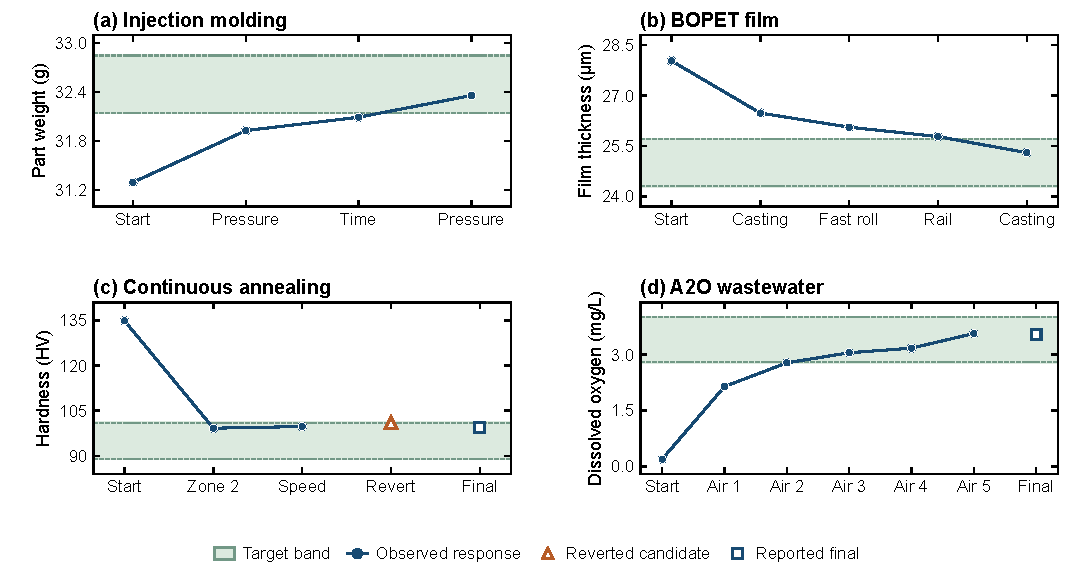
\includegraphics[width=\textwidth]{resources/fig-missions-origin.pdf}
\caption{Process observations from four simulated missions. Shading denotes
the scenario-specific target band and circles denote structured trajectory
observations, joined to indicate order only. The open triangle marks the annealing candidate that was
reverted; its value comes from event text rather than a structured trajectory
record. Open squares show separately reported mission-final values for
annealing and wastewater; these are not connected to the preceding
observations. Horizontal positions indicate event order, not elapsed time.
Each panel represents one deterministic trajectory.}
\label{fig:missions}
\end{figure*}

\subsection{Injection Molding and Film Thickness}
The injection-molding mission targeted $32.5\pm0.35$\,g. Starting at
31.296\,g, the routine requested holding pressure from 45 to 57.73\,bar and
holding time from 6 to 10.56\,s; observations rose to 31.93 and 32.09\,g.
A further pressure request to 62\,bar preceded the final 32.36\,g observation
within the target band. This single sequence does not isolate the effect of
each parameter.

The BOPET mission targeted $25.0\pm0.7$\,$\mu$m. From an initial
28.03\,$\mu$m, four requests changed casting speed, fast-roll speed, rail
width, and casting speed again; successive observations were 26.48, 26.06,
25.78, and 25.30\,$\mu$m. The final value was within the band, while the
first three remained above it. Reported melt temperatures were
291.3--291.8\,$^{\circ}$C, within the configured 268--300\,$^{\circ}$C
window. These observations describe one simulated sequence.

\subsection{Annealing and Wastewater Treatment}
The annealing mission combined a $95\pm6$\,HV hardness target with a
line-speed increase. From 134.9\,HV, a zone-2 temperature request from 710 to
850\,$^{\circ}$C preceded a structured observation of 99.18\,HV; a speed
request from 140 to 152\,m/min preceded 99.74\,HV. A 164\,m/min candidate
was reverted after event text reported 101.0\,HV, at the upper target boundary
and outside the configured margin. The summary separately reported final
hardness of 99.5\,HV and retained speed of 152\,m/min, 8.57\% above the initial
setting, not a measured throughput gain. A zone-3 read failed before the
zone-2 action. Final tensile-strength and surface-defect measurements were
not archived, so the record cannot establish that all quality constraints
were met.

The wastewater mission targeted dissolved oxygen (DO) at $3.4\pm0.6$\,mg/L.
Five blower-frequency increases from 26 to 34.1\,Hz accompanied a rise from
0.194 to 3.567\,mg/L in the structured aeration sequence. Subsequent alkali
and coagulant dosing addressed pH and phosphorus; observed total phosphorus
fell from 0.662 to 0.5507, 0.4607, and 0.413\,mg/L. A later blower reduction
was reverted after insufficient margin. The summary separately reported final
DO of 3.54\,mg/L and a simulator-defined cost index changing from 182.6 to
180.2, not a measured operating cost. The complete final effluent vector was
not archived, so these values do not verify all discharge constraints.

\subsection{Evidence Synthesis}
Each mission's reported final primary variable lies within its target band,
whereas the separate harness probes remained below their respective targets.
The protocol, onboarding, entry-path, and mock approval checks address
different questions and are not combined with the process trajectories. These
results do not establish repeatability, causal effects of individual actions,
comparative performance, human-approval effectiveness, or transfer to a
physical plant.
